\subsection{Martin Andleberger}
\begin{center}
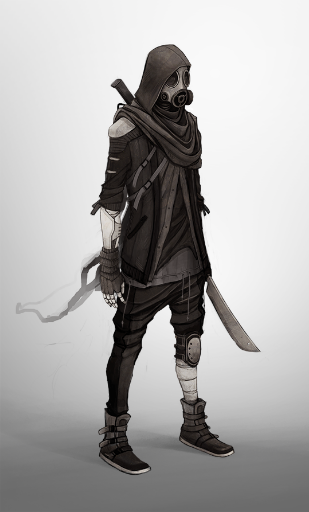
\includegraphics[width=80mm]{./content/img/martin.png}
\begin{figure}[h]
\end{figure}
\end{center}

\textbf{Details}\\
Race: Construct\\
Class: Bard/Sorcerer\\
Age: 87\\
Status: Possibly a Mouse\bigskip

\textbf{Background}\\
The AndelBergers seemed like any other old aristocratic family from Lindedorf, at least from the outside. Who was to know that the family line stretched almost a 1000 years back in history. So far back that the families histories pre-dated the sundering itself.    \medskip

Lord and Lady AndelBergers had been (in)breeding their family ever since the sundering to maintain a pure bloodline, the latest incarnation had proved very difficult indeed as the Lady had only managed to produce a single child, a solitary lady who glowed with the radiance of Hemotate. She was schooled from the families great library and a sense of destiny passed into her. Until one dark and stormy night the church arrived, or at least a part of the church that people only talked about in whispers. Dark masked figures stormed the house and decimated what was left of the family, what happened to the young Ms AndelBerger is still unknown.   \medskip

MarTin was the family butler, built to protect and serve Ms AndelBerger and keep her entertained. He had been fashioned using the knowledge of the ancient family line, his clothes and parts shaped in strange swirling patterns taken from books long useless. On the fateful night the inquisition appeared, Martin was out milking the cows in the freezing rain. He missed the entire saga, only returning to an empty house torn apart at the seems. He rescued his favourite books, and weighed up his options. He had lost everything, but he still had two purposes, to find the young Ms AndelBerger, and to avenge the family line. As possibly the last member of the family line it was now up to him to return the gods to their rightful place within the pantheon.    \medskip

All this was almost a century ago, MarTin has been wandering ever since    \medskip

Unable to die the butler wandered the streets, then the town, then the city, until finally the continent. Until he was chanced upon by a motley crew in an airship....     

\textbf{Personality and Traits}\\
Martin was very depressed, and lacked the spark of power that helps him deal with the day to day drudgery of being immortal. When he discovered the teams goals were to destroy the church he picked himself up only a little bit. It wasn't until he discovered that his ward Ms Andelberger was gone, and ascended to the heavens, that he doubled down and vowed vengeance
Speaks Tikki Tuck, Goblin, and Low Velterran    

\textbf{Relationships}
Martin is forming relationships within the team, he seems most attached to Burnie.\bigskip

\clearpage